% from manual https://www.researchgate.net/profile/Juergen_Hackl/publication/319894904_TikZ-network_manual/links/59cb46e2a6fdcc451d5c91ff/TikZ-network-manual.pdf?origin=publication_detail

\documentclass[tikz,border=5]{standalone}
\usepackage{tikz-network}     % tikz-network.sty file must be present

\begin{document} 
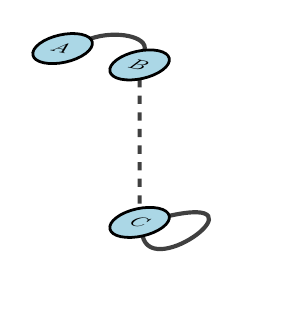
\begin{tikzpicture}[multilayer=3d]
    \Vertex[x=0.5,IdAsLabel,layer=1]{A}
    \Vertex[x=1.5,IdAsLabel,layer=1]{B}
    \Vertex[x=1.5,IdAsLabel,layer=2]{C}
    \Edge[bend=60](A)(B)
    \Edge[style=dashed](B)(C)
    \Edge(C)(C)

\end{tikzpicture}
\end{document} 